\section{Group Contribution}

\begin{table}[h]
\begin{tabular}{|c|c|c|}
\hline
\textbf{Group Member} & \textbf{UID} & \textbf{Contribution}\\
\hline
Tong Cheuk Yin & 3036068503 & 33.3\% \\
\hline
Wong Tsz Yui & 3036293196 & 33.3\% \\
\hline
Yeo Wei Jie David & 3036677990 & 33.3\% \\
\hline
\end{tabular}
\end{table}

\section{Data Visualization}

\begin{figure}[h]
    \centering
    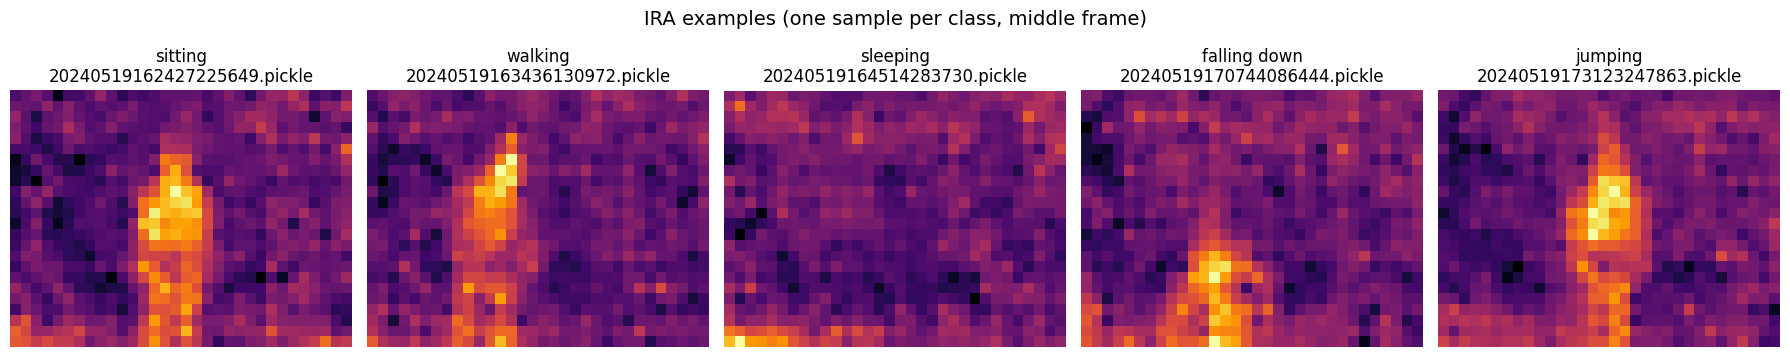
\includegraphics[width=1\linewidth]{fig/visualization_ira.png}
    \caption{Visualization of IRA Samples}
    \label{fig:placeholder}
\end{figure}

IRA samples used:

  1 - sitting: 20240519162427225649.pickle
  
  2 - walking: 20240519163436130972.pickle
  
  3 - sleeping: 20240519164514283730.pickle
  
  4 - falling down: 20240519170744086444.pickle
  
  5 - jumping: 20240519173123247863.pickle

\begin{figure}[h]
    \centering
    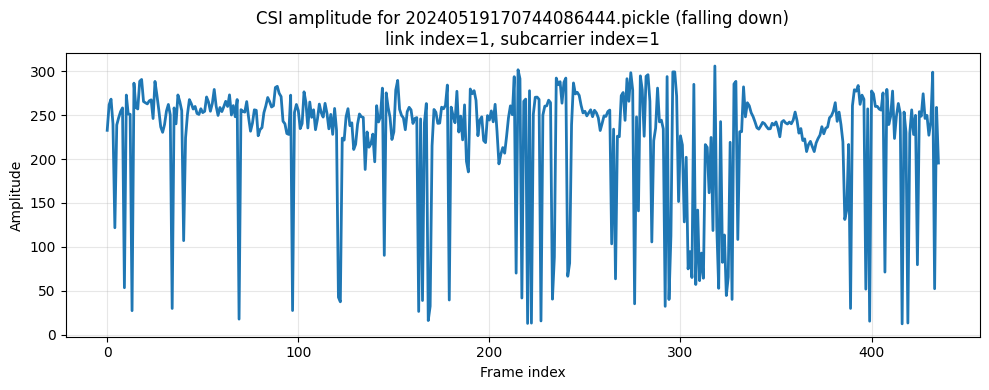
\includegraphics[width=1\linewidth]{fig/visualization_csi.png}
    \caption{Visualization of CSI Amplitude}
    \label{fig:placeholder}
\end{figure}

CSI sample used:

  20240519170744086444.pickle (falling down), link index=1, subcarrier index=1

\section{Preprocessing}
All three modalities i.e. Infrared Array (IRA), WiFi CSI, and IMU, are stored in pickle files that contain both raw sensor frames and associated timestamps. A common preprocessing pipeline is applied to all samples before training any models, so as to ensure consistent input dimensions and temporal alignment across the models.

\subsection{Data Loading}
The original pickle files were created with an older version of pandas and they contain references to \\
\verb|pandas._libs.tslibs.timestamps|. To make them loadable in any environment, a custom \verb|CompatUnpickler| overrides the \verb|find_class| method to redirect the timestamp unpickling routine to a simple converter that returns a standard Python \verb|datetime|. Additionally, references to \verb|numpy._core| are mapped to \verb|numpy.core| for broader NumPy version compatibilities.

\subsection{Temporal Alignment & Resampling}
Each modality records frames at their own sampling rate. The timestamps are also not perfectly synchronised. To obtain a consistent input for the models, the following steps were implemented for each sample:

\begin{enumerate}
	\item For every model, the first valid node is selected (i.e. a sensor stream with non-empty frames). Missing modalities are replaced by zero-valued tensors of the expected shape.
	\item Timestamps are cleaned and converted into nanoseconds. Invalid or missing timestamps are discarded.
	\item When at least two modalities contain valid timestamps, a shared timeline is constructed as the overlapping time interval between the earliest end and the latest start among them. The timeline is then uniformly resampled to a fixed number of frames:
	\begin{itemize}
		\item IRA: 24 frames
		\item CSI: 48 frames
		\item IMU: 64 frames
	\end{itemize}
	\item If there is no overlap, each modality is resampled independently to the target length, using linear index interpolation.
	\item Nearest-neighbor lookup is used on the original timestamp arrays, for alignment to the shared timeline.
\end{enumerate}

\subsection{Normalization & Feature Engineering}
After alignment, the raw frames of each modality are normalized to have zero mean and unit variance. For the IRA data, this normalization is computed globally across all pixels and frames within the sample. For CSI and IMU data, normalization is computed along the temporal axis.

For CSI and IMU, additional features are derived to capture dynamic changes:
\begin{itemize}
	\item For WiFi CSI, the complex-valued frames are converted to amplitude by taking the absolute value. A first-order difference (delta) is computed along the time dimension to show the rate of change of the channel state. This delta array is independently normalized, and then the amplitude and delta arrays are concatenated along the channel axis, resulting in a 4-channel input (2 original links \times 2 features).
	\item For IMU, a delta feature is also computed from the normalized frames. The original frames and delta frames are stacked to form a 2-channel 3D tensor (channel 0: raw, 1: delta).
\end{itemize}

All tensors are finally cast to \texttt{float32}. To avoid extreme values from sensor noise, the normalized CSI and IMU tensors are clipped to the range [-5, 5].

\section{Single Modality Models}

\subsection{Model Design and Implementation Details}

\subsubsection{IRA Model}

The neural network for the IRA Model uses a 3D convolutional neural network (3D CNN). Similar to the IMU model, the structure is mainly divided into two parts: feature extraction and classification.

\textbf{\underline{Feature Extraction}}

This part of the network extracts spatial and temporal features from the IRA thermal frames. It consists of the following layers:
\begin{itemize}
    \item 3D Convolution
    \item 3D Batch Normalization
    \item Rectified Linear Unit (ReLU) Activation
    \item 3D Max Pooling
    \item 3D Adaptive Average Pooling (final layer)
\end{itemize}

The IRA data is represented as a 4D tensor with dimensions (time height width). Subsequently after adding a channel dimension it becomes (1, time, height, width). A 3D CNN is suitable for this modality, because it can simultaneously capture: how the thermal signature evolves over the 24‑frame sequence (temporal dynamics); and the 2D heat distribution (24\(\times\)32 pixels) that characterizes different postures and movements (spatial patterns).

BatchNorm is applied after each convolution to stabilize activations and to accelerate convergence. ReLU is used as the activation function due to its simplicity and effectiveness in mitigating vanishing gradients, which is important for the relatively shallow network used in this case.

Max pooling layers progressively reduce the spatial and temporal resolution. This forces the network to retain only the most prominent features, while reducing computational load. The final layer of the feature extractor is an Adaptive Average Pooling layer that collapses the remaining feature maps to a fixed spatial size of (1, 1, 1). A compact 128‑dimensional vector is produced, which summarizes the entire IRA sequence.

\textbf{\underline{Classifier}}

The classifier portion converts the 128‑dimensional feature vector into activity class predictions. It contains:
\begin{itemize}
    \item Flatten
    \item Dropout (rate 0.30)
    \item Linear layer (128 \(\rightarrow\) 64)
    \item ReLU Activation
    \item Dropout (rate 0.20)
    \item Linear layer (64 \(\rightarrow\) 5)
\end{itemize}

Since the IRA model is trained on only 400 samples, dropout is employed to reduce overfitting. The two‑stage linear reduction (128\(\rightarrow\)64\(\rightarrow\)5) provides a non‑linear decision boundary while keeping the number of parameters manageable.


\subsubsection{CSI Model}

The CSI Model processes WiFi Channel State Information , through using a 2D convolutional neural network (2D CNN). Unlike IRA and IMU, CSI data is represented as a 3D tensor with dimensions (time links and subcarriers). The model follows the same two‑part structure: feature extraction and classification.

\textbf{\underline{Feature Extraction}}

The feature extraction block operates on a 4‑channel input constructed from the preprocessed CSI frames. The layers include:
\begin{itemize}
    \item 2D Convolution (with bias disabled)
    \item 2D Batch Normalization
    \item Gaussian Error Linear Unit (GELU) Activation
    \item 2D Max Pooling
    \item 2D Adaptive Average Pooling (final layer)
\end{itemize}

A 2D CNN is chosen because the two spatial axes of the CSI tensor (links (2 receiving antennas) and subcarriers (114 frequency bins)) form a structured grid. This allows the model to learn frequency selective and antenna specific patterns. The time axis is also treated as the channel dimension of the 2D feature maps after the initial feature stacking (amplitude + delta). It enables the convolutions to operate together on the time‑varying spectral information.

GELU activation is used for the similar reasons as in the IMU model, as it provides a smoother non‑linearity that can better capture subtle variations in the CSI amplitude and delta signals. Max pooling reduces the spatial dimensions (links and subcarriers) progressively, while Adaptive Average Pooling compresses the final feature maps to a fixed size of (3, 6), resulting in a flattened vector of length \(192 \times 3 \times 6 = 3456\).

\textbf{\underline{Classifier}}

The classifier consists of:
\begin{itemize}
    \item Flatten
    \item Dropout (rate 0.25)
    \item LazyLinear (output 256)
    \item GELU Activation
    \item Dropout (rate 0.20)
    \item Linear layer (256 \(\rightarrow\) 5)
\end{itemize}

A LazyLinear layer is used to automatically infer the input size from the preceding adaptive pooling output, which simplifies architectural changes during development. The two dropout layers with moderate rates (0.25 and 0.20) help prevent overfitting given the limited dataset size, while the GELU activation maintains consistency with the feature extraction block.


\subsubsection{IMU Model}
The Neural Network for the IMU Model uses a 3D convolution neural network (3D CNN). The model is split into 2 portions, feature extraction and classification.

\textbf{\underline{Feature Extraction}}

This portion of the neural network extracts useful features from the IMU data.

This portion includes the following layers:
\begin{itemize}
    \item 3D Convolution 
    \item 3D Batch Normalization
    \item Gaussian Error Linear Unit (GELU) Activation Function
    \item 3D Max Pooling (for some layers)
    \item 3D Adaptive Average Pooling (for the last layer)
\end{itemize}

3D CNNs are used because the IMU data is represented as a structured 3D tensor with dimensions corresponding to time, the IMU feature-channel dimension, and the IMU node or joint dimension. After preprocessing, the model can convolve across these three dimensions simultaneously, allowing it to learn local spatiotemporal patterns from the data. This is well suited to human activity recognition, since activities are defined not only by motion over time but also by coordinated movement across different body regions, which is reflected in the measurements recorded at different feature channels and IMU nodes.

Batch Normalization is used to stabilize the distribution of intermediate activations during training. This is appropriate for IMU data because inertial measurements can vary substantially across samples. As a result, Batch Normalization helps make training more stable, improves convergence speed, and reduces sensitivity to differences in signal scale.

GELU is used as the activation function because it provides a smoother nonlinear transformation than ReLU. This is beneficial for IMU data, where small but meaningful motion patterns may be important for distinguishing activities. The smoother behaviour of GELU can help the network learn subtle relationships more effectively, especially when combined with normalized activations from the Batch Normalization layers.

Max-pooling layers are applied after groups of 3D convolution layers to progressively downsample the feature maps. They reduce the spatial and temporal resolution after features have already been learned by the convolution layers. This helps the network retain the most important responses, reduce computational cost, and gradually build higher-level spatiotemporal representations of the IMU signal.

The final layer of the feature extraction block is an Adaptive Average Pooling layer. This layer compresses the learned feature maps into a fixed output size, producing a compact representation of the IMU sequence. This fixed-size representation is then passed to the classifier portion of the model, which uses it to predict the final activity class.

\textbf{\underline{Classifier}}

The portion of the IMU Model converts the extracted feature representation from the Feature Extraction portion into the final activity labels.

This portion includes the following layers:
\begin{itemize}
    \item Flatten 
    \item Dropout
    \item LazyLinear
    \item Gaussian Error Linear Unit (GELU) Activation Function
    \item Linear
\end{itemize}

The output of the feature extraction block is first compressed into a fixed-size representation and then flattened into a one-dimensional feature vector. This converts the learned spatiotemporal feature maps into a format that can be processed by the fully connected classifier layers.

Dropout layers are used to reduce overfitting by randomly deactivating a proportion of neurons during training. This encourages the model to rely on a broader set of learned features, rather than depending too heavily on only a small number of activations for classification.

A LazyLinear layer is used instead of a standard Linear layer because it can automatically infer the input dimensionality from the flattened feature vector during the first forward pass. This is convenient because the exact size of the flattened representation depends on the output shape of the preceding feature extraction block.

The final Linear layer maps the classifier representation to the five output classes. It produces one score for each activity class, and these scores are then used to determine the predicted label for the IMU sample.

\subsection{Runtime}

Overall, the number of training epochs required to find the best modality classifier for each single modality is shown below:

\begin{figure}[h]
    \centering
    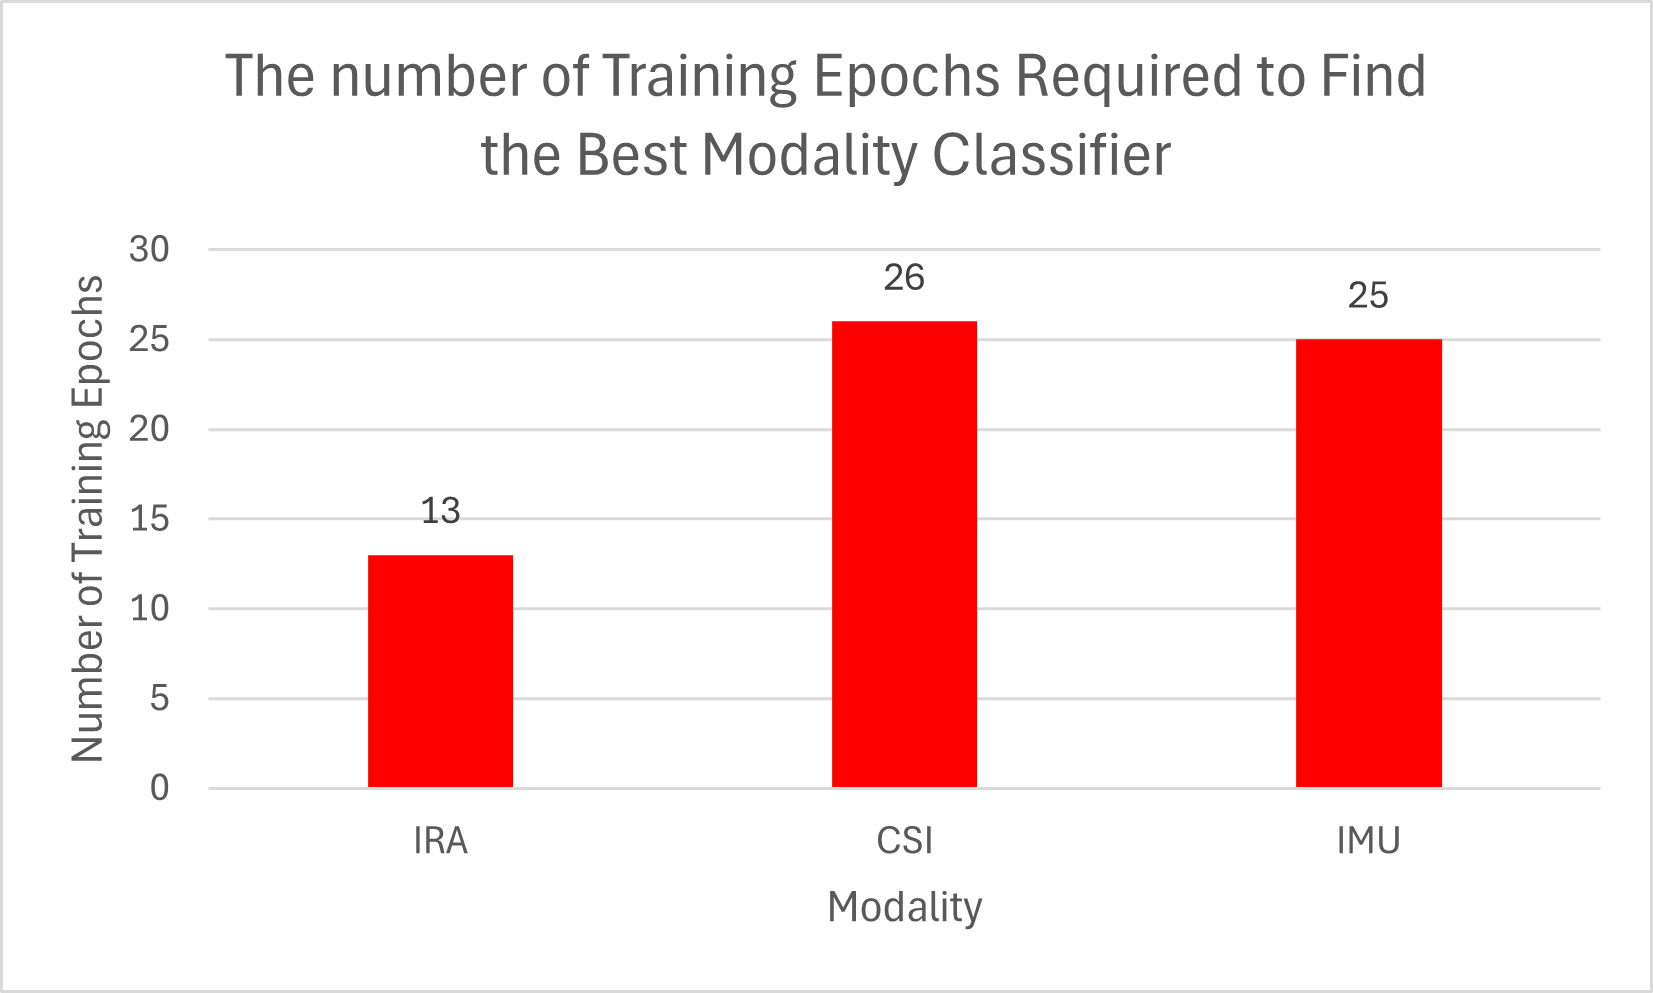
\includegraphics[width=1\linewidth]{fig/single_num_epoch_best_clf.png}
    \caption{The number of Training Epochs Required to Find the Best Modality Classifier}
    \label{fig:placeholder}
\end{figure}

For each single modality, the number of training epochs required to find the best modality classifier (the modality classifier with highest validation accuracy) and the total number of training epochs are reported as below:

\subsubsection{IRA Modality Classifier}

The best IRA modality classifier is found in the 13th training epoch. In total, the training of IRA modality classifier took 19 epochs with the early stopping triggered.

\subsubsection{CSI Modality Classifier}

The best CSI modality classifier is found in the 26th training epoch. In total, the training of CSI modality classifier took 30 epochs with the maximum number of epochs reached.

\subsubsection{IMU Modality Classifier}

The best IMU modality classifier is found in the 25th training epoch. In total, the training of IMU modality classifier took 25 epochs with the maximum number of epochs reached.

\subsection{Training/Validation Loss Curves (figures)}

For each single modality, the validation accuracy of the best modality classifier, the loss curve, and the accuracy curve is reported as below:

\subsubsection{IRA Modality Classifier}

The validation accuracy of the best IRA modality classifier is 0.9250, and is found in the 13th training epoch:

\begin{figure}[h]
    \centering
    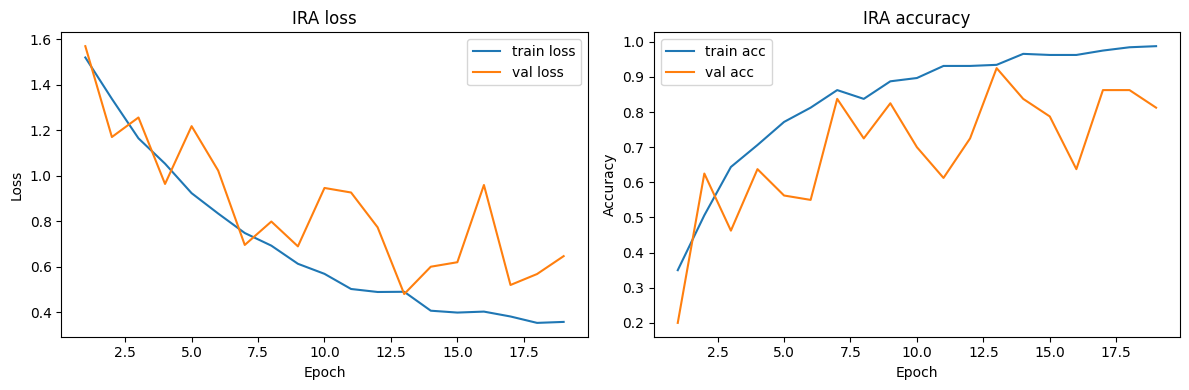
\includegraphics[width=1\linewidth]{fig/loss_accuracy_ira.png}
    \caption{IRA Loss and Accuracy}
    \label{fig:placeholder}
\end{figure}

\subsubsection{CSI Modality Classifier}

The validation accuracy of the best CSI modality classifier is 0.7500, and is found in the 26th training epoch:

\begin{figure}[h]
    \centering
    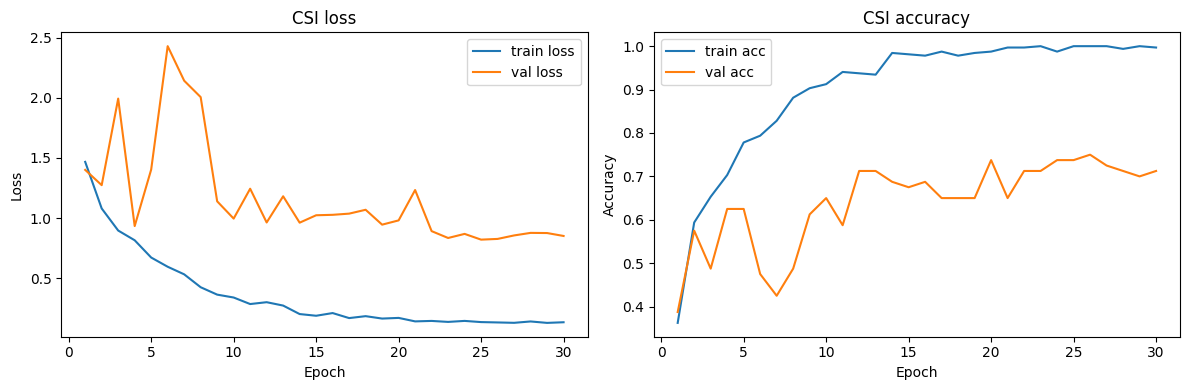
\includegraphics[width=1\linewidth]{fig/loss_accuracy_csi.png}
    \caption{CSI Loss and Accuracy}
    \label{fig:placeholder}
\end{figure}

\subsubsection{IMU Modality Classifier}

The validation accuracy of the best IMU modality classifier is 1.0000, and is found in the 25th training epoch:

\begin{figure}[h]
    \centering
    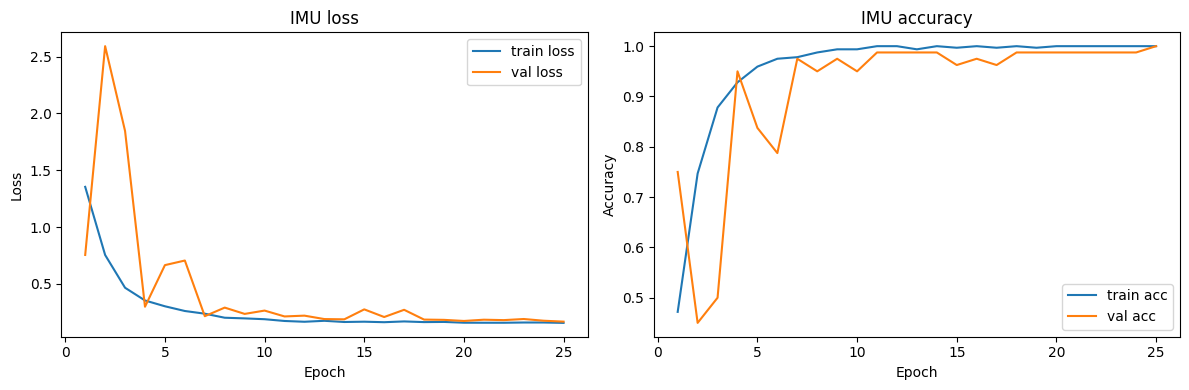
\includegraphics[width=1\linewidth]{fig/loss_accuracy_imu.png}
    \caption{IMU Loss and Accuracy}
    \label{fig:placeholder}
\end{figure}

\subsection{Discussion and Analysis of Validation Results}

The IRA modality classifier achieves a strong validation accuracy of 92.5\%. This is reasonable, as the IRA sample, as shown in Figure 1, is similar to a regular photograph, in which humans can use visual perception to easily identify the pose inside the “picture”.

In the IRA modality classifier, CNN is used, which has been proved a strong image classifier. Therefore, by applying CNN on the IRA samples, we may expect a performance that is as strong as a CNN image classifier. Technically speaking, the spatial and temporal convolution may allow the model to learn posture-related heat distributions and motion-related thermal evolution.

The CSI model achieves a lower validation accuracy of 75.0\%, making it the weakest standalone modality. The reason might be that the measured CSI contains significant noises from SFO, CFO, etc. The present of noise may be confirmed by the small but consistent high-frequency fluctuations in the CSI amplitude that has been visualized in Figure 2.

In addition to the small training dataset containing only 320 samples, the CSI model may be overfit to the noise. Such deduction echoes with the significant gap between the training accuracy and the validation accuracy revealed in the accuracy curve, where towards the end of the training, the training accuracy is near 1.0, but the validation accuracy is capped at 0.75.

The IMU modality classifier achieves 100\% validation accuracy, indicating that inertial data is extremely informative for the activities considered. In fact, distinctive sensor patterns are produced from different activities:
\begin{itemize}
    \item Sit: IMU signals are stable with near‑constant acceleration from gravity and almost zero rotational movement.
    \item Walk: IMU data shows regular, periodic acceleration and rotation patterns corresponding to steps.
    \item Sleep: IMU signals remain nearly constant for long periods with very low variance and minimal movement.
    \item Falldown: IMU sensors capture a sudden, high‑magnitude acceleration and rotation spike followed by inactivity.
    \item Jump: IMU data exhibits a short burst of strong acceleration with a brief low‑acceleration airborne phase and a landing impact.
\end{itemize}
The unique signal signature from each activity enables easy learning.

\section{Multi Modality Models}

\subsection{Model Design and Implementation Details}
The combined model follows a multimodal late-fusion architecture. It contains three modality-specific branches, one each for IRA, CSI, and IMU, which process their respective input samples independently. The outputs of these three branches are then combined and passed to a shared classifier to predict the final activity class.

More specifically, each modality-specific branch is divided into two parts: a feature extraction component and a projection component. The feature extraction component serves the same role as in the single-modality models discussed earlier, namely to learn meaningful modality-specific patterns from the raw input data. However, instead of ending with a classification head, each branch uses a projection layer that transforms its extracted features into a compact 64-dimensional embedding vector.

These three 64-dimensional embedding vectors, one from each modality, are then concatenated to form a single 192-dimensional fused representation. This fused vector is passed into a classifier composed of Linear layers, which produces the final prediction across the five activity classes.

\subsection{Runtime}

The best multi modality classifier is found in the 7th training epoch. In total, the training of multi modality classifier took 20 epochs with the maximum number of epochs reached.

Overall, the number of training epochs required to find the best modality classifier for each modality is shown below:

\begin{figure}[h]
    \centering
    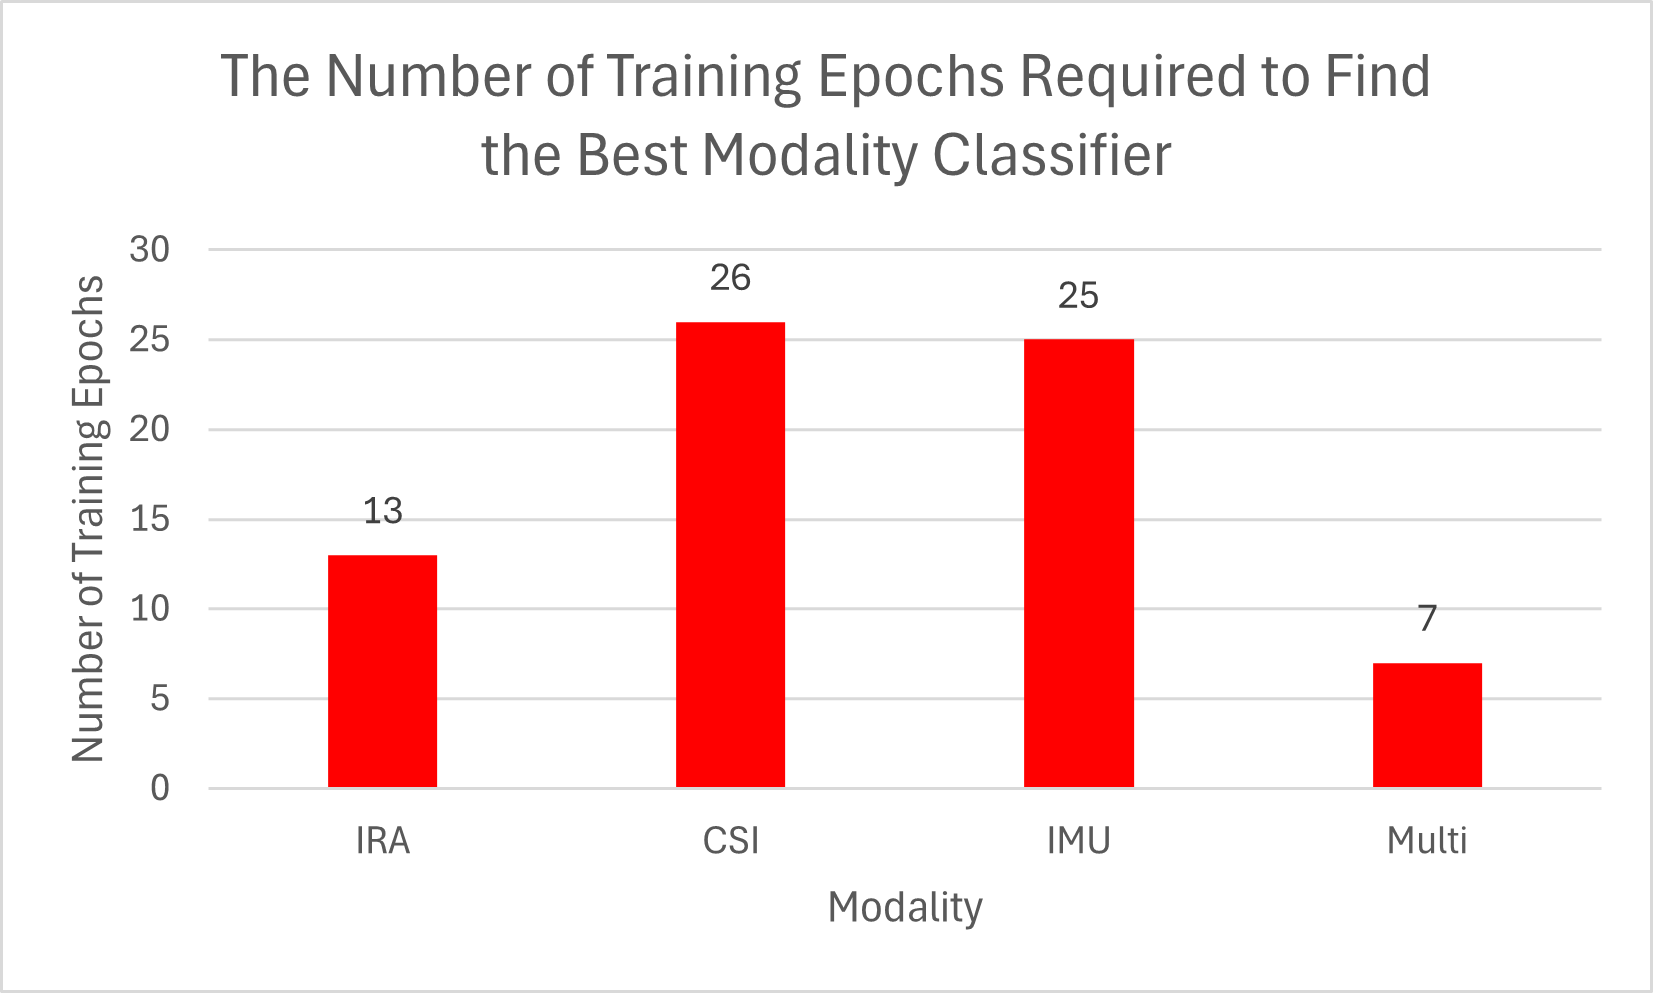
\includegraphics[width=1\linewidth]{fig/num_epoch_best_clf.png}
    \caption{The number of Training Epochs Required to Find the Best Modality Classifier}
    \label{fig:placeholder}
\end{figure}

\subsection{Training/Validation Loss Curves (figures)}

The validation accuracy of the best multi modality classifier is 1.0000, and is found in the 7th training epoch:

\begin{figure}[h]
    \centering
    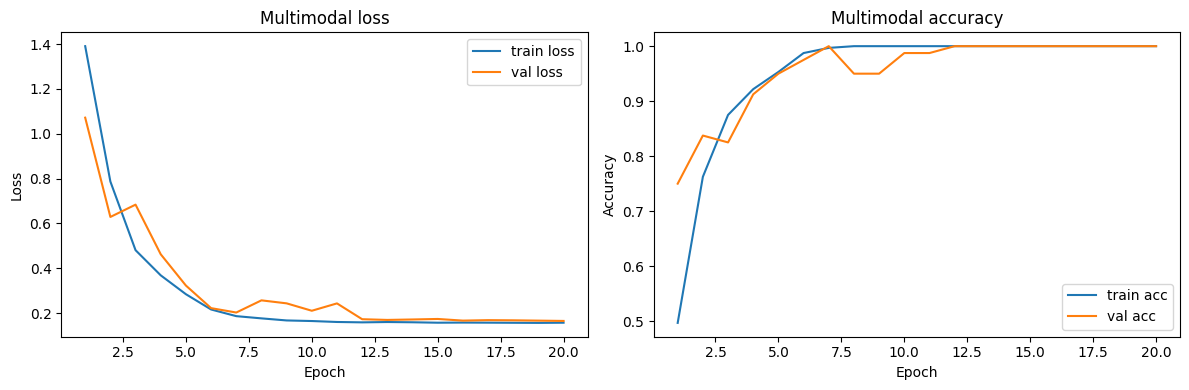
\includegraphics[width=1\linewidth]{fig/loss_accuracy_multi.png}
    \caption{Multi Modality Loss and Accuracy}
    \label{fig:placeholder}
\end{figure}

\subsection{Discussion and Analysis of Validation Results}

The combined multimodal classifier also reaches 100\% validation accuracy, and notably does so much earlier (epoch 7) than the single-modality models. This rapid convergence indicates that the fused representation is highly discriminative and easier for the classifier to separate. This result is unsurprising, as the ensemble classifier is not expected to perform worse than its strongest constituent model—in this case, the IMU modality classifier, which achieved 100\% validation accuracy. On the other hand, fastest convergence among the 4 modality classifiers can be credited to the classification ability boosted by ensembling independent classifiers.

\section{Conclusion}

Overall, the validation accuracy of the best modality classifier for each modality is shown below:

\begin{figure}[h]
    \centering
    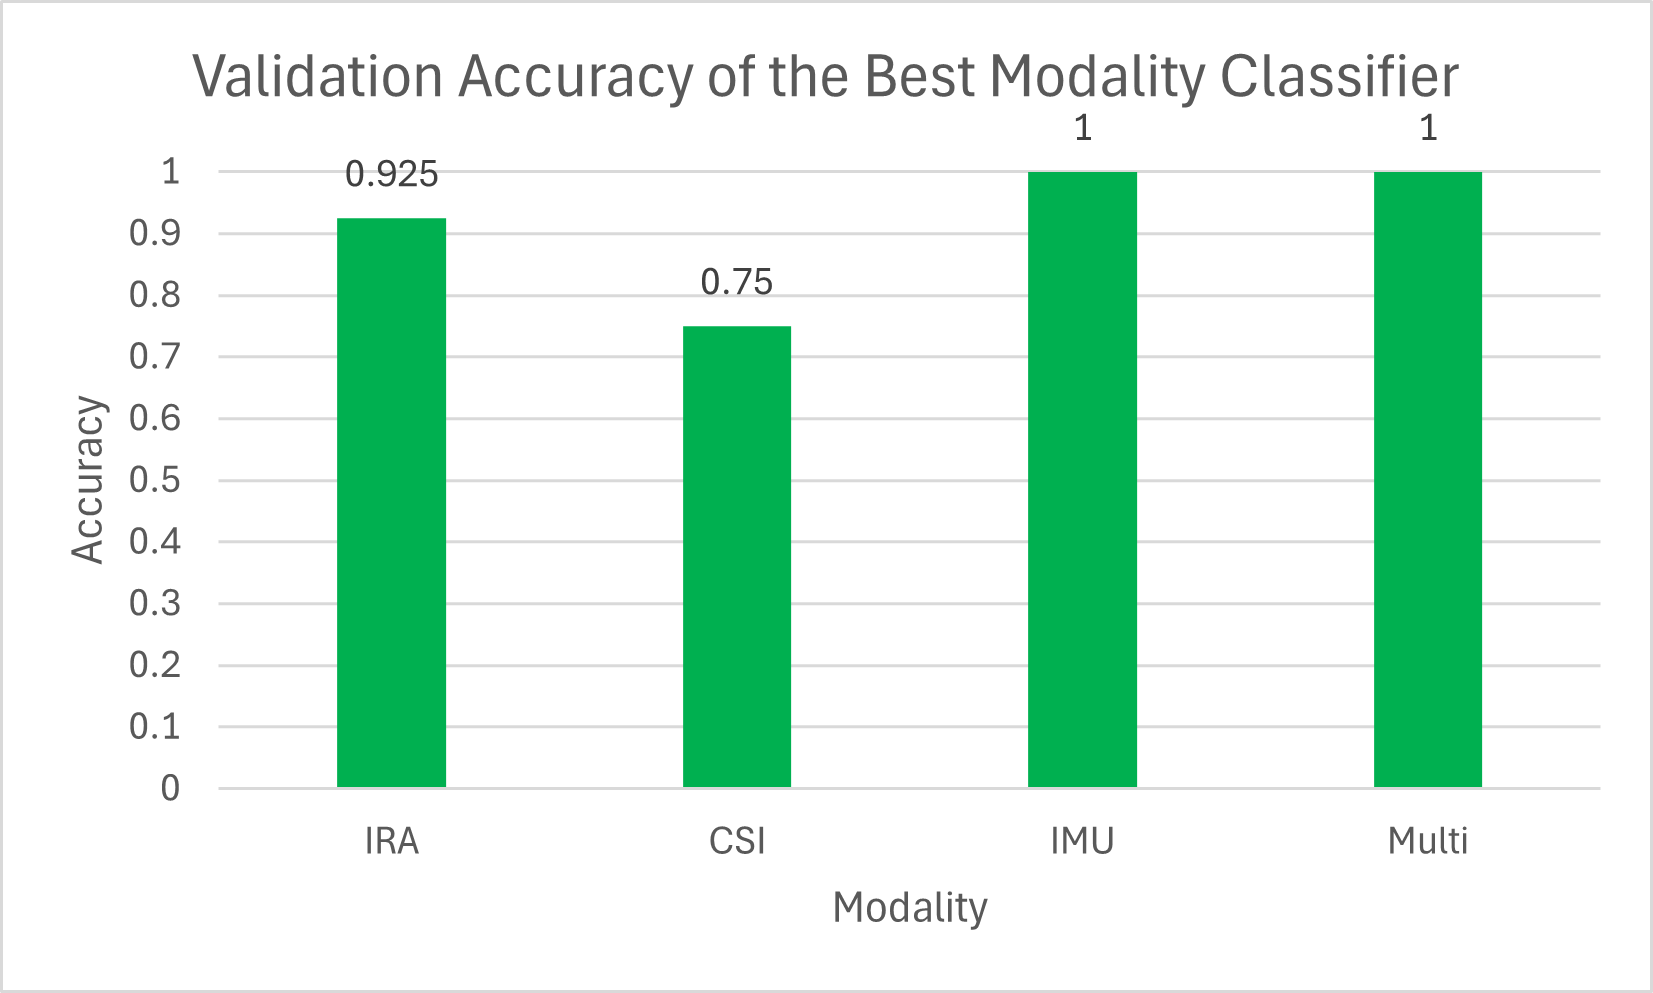
\includegraphics[width=1\linewidth]{fig/val_acc_best_modal_clf.png}
    \caption{Validation Accuracy of the Best Modality Classifier}
    \label{fig:placeholder}
\end{figure}

In summary, IMU is the most informative single modality, achieving perfect validation accuracy. IRA provides strong complementary spatial-temporal cues, with high accuracy and fast convergence. CSI alone is less reliable, but still contributes valuable information when fused.
